\chapter{Logistic Regression}

In the workflow above we have used logistic regression, a popular machine learning method. It is often used in text mining for its speed and predictive performance. How does it work?

\marginnote{This visualization is called a nomogram. It displays scores (votes) of each attribute for the selected target value at the top left.}It lets the words vote. For example, the word 'fox' in the text votes for the tale being an animal tale. So do cats and birds and wolves, but not so strongly (lines in the visualization are much shorter). We can see that the word 'fox' is the best clue for the text being an animal tale.

\vspace{-0.2cm}
\begin{figure*}[h]
  \centering
  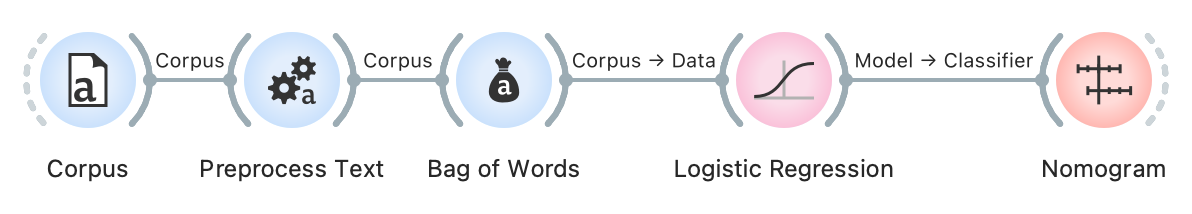
\includegraphics[width=0.8\linewidth]{workflow.png}%
  \caption{$\;$}
\end{figure*}
\vspace{-0.3cm}

The word 'little' votes for the opposition. So does 'came' (see how they have zeros at the right end of the scale?). The more little things there are in a story, the less likely it is an animal tale.

\marginnote{In Nomogram, you can interactively observe the model's classification. Drag the blue dots left or right so that the accumulated sum of points (Total) is as high as possible.}Each word gives a score. If there are 29 foxes in the text, then the model will give it 3 points for being an animal tale. And if there are no words 'little', it will give it an additional 4.5 points.

Of course the real method is a bit more complicated - it tries to find appropriate vote weights and thresholds. But this involves some linear algebra and other scarier-than-wolves words, so let's not stroll down this path.

\vspace{-0.2cm}
\begin{figure*}[h]
  \centering
  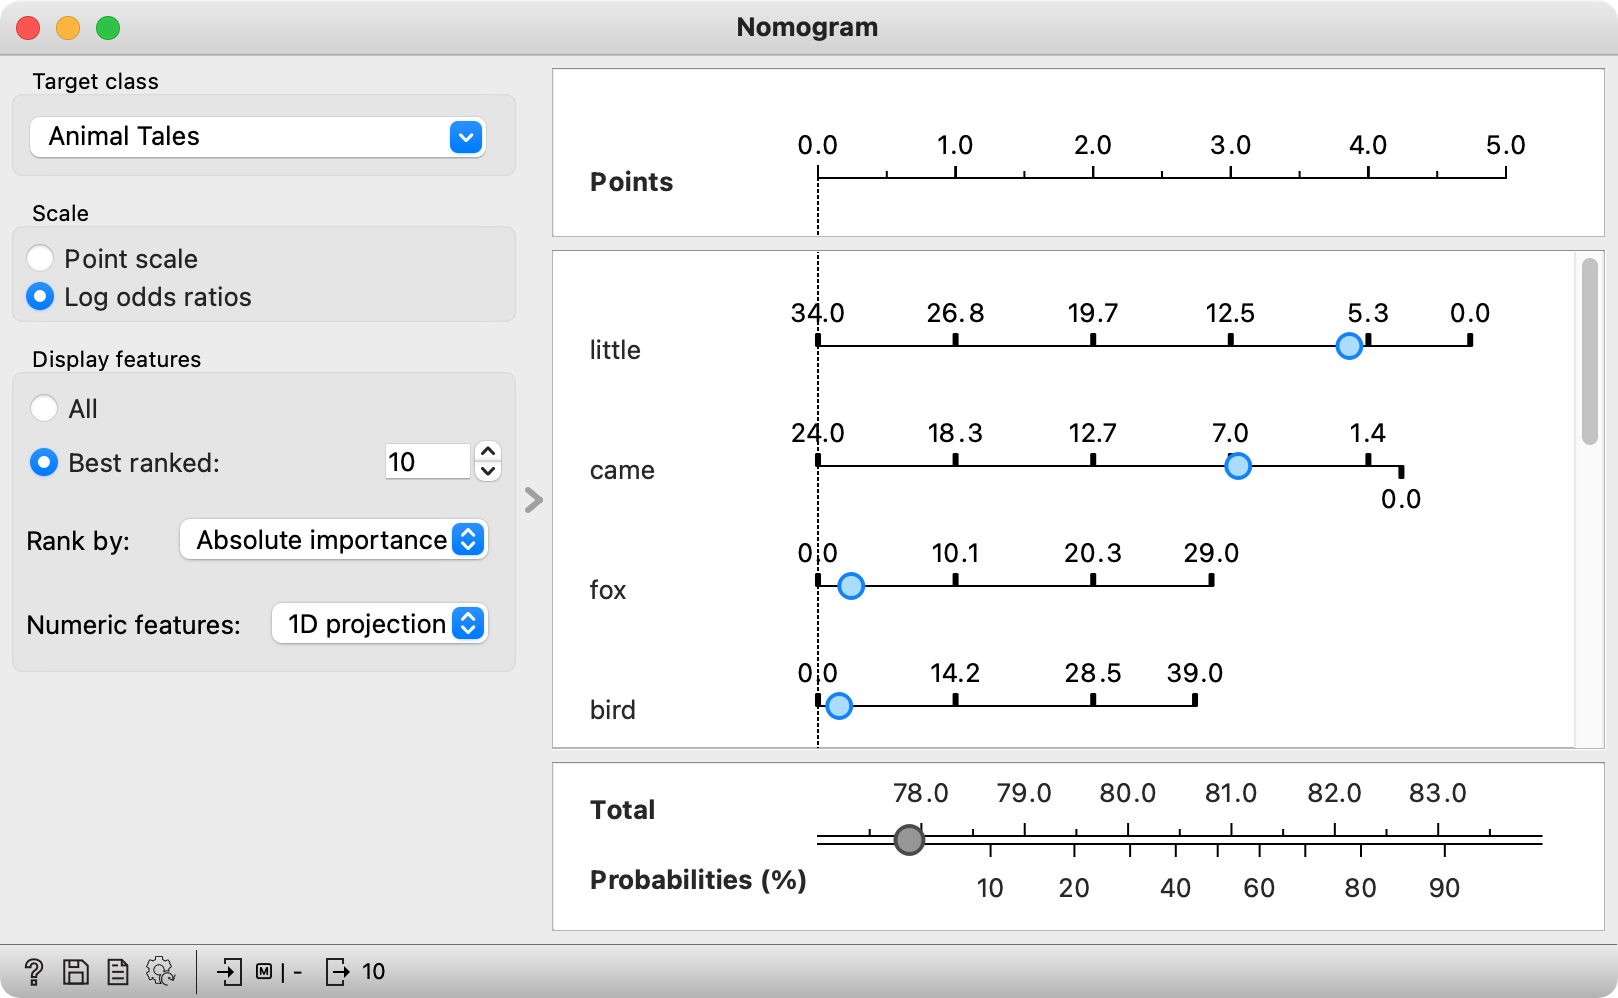
\includegraphics[width=0.8\linewidth]{nomogram.png}%
  \caption{$\;$}
\end{figure*}
\vspace{-0.3cm}
